\documentclass[12pt,a4paper]{article}
\usepackage[top=1.5cm, bottom=1.5cm, left=2.0cm, right=1.5cm] {geometry}
\usepackage{amsmath,amssymb,fontawesome}
\usepackage{tkz-euclide}
\usepackage{setspace}
\usepackage{lastpage}

\usepackage{tikz,tkz-tab}
%\usepackage[solcolor]{ex_test}
\usepackage[dethi]{ex_test} % Chỉ hiển thị đề thi
%\usepackage[loigiai]{ex_test} % Hiển thị lời giải
%\usepackage[color]{ex_test} % Khoanh các đáp án
\usetikzlibrary{shapes.geometric,arrows,calc,intersections,angles,quotes,patterns,snakes,positioning}
\everymath{\displaystyle}

\def\colorEX{\color{purple}}
%\def\colorEX{}%Không tô màu đáp án đúng trong tùy chọn loigiai
\renewtheorem{ex}{\color{violet}Câu}
\renewcommand{\FalseEX}{\stepcounter{dapan}{{\bf \textcolor{blue}{\Alph{dapan}.}}}}
\renewcommand{\TrueEX}{\stepcounter{dapan}{{\bf \textcolor{blue}{\Alph{dapan}.}}}}

%---------- Khai báo viết tắt, in đáp án
\newcommand{\hoac}[1]{ %hệ hoặc
    \left[\begin{aligned}#1\end{aligned}\right.}
\newcommand{\heva}[1]{ %hệ và
    \left\{\begin{aligned}#1\end{aligned}\right.}

%Tiêu đề
\newcommand{\tenso}{iMath}
\newcommand{\tentruong}{0974.940.049}
\newcommand{\tenkythi}{ĐỀ ÔN TẬP}
\newcommand{\tenmonthi}{Môn học: TOÁN 10}
\newcommand{\thoigian}{}
\newcommand{\tieude}[1]{
    \noindent
     \begin{minipage}[b]{6cm}
    \centerline{\textbf{\fontsize{11}{0}\selectfont \tenso}}
    \centerline{\fontsize{11}{0}\selectfont \tentruong}  
  \end{minipage}\hspace{1cm}
  \begin{minipage}[b]{11cm}
    \centerline{\textbf{\fontsize{11}{0}\selectfont \tenkythi}}
    \centerline{\textbf{\fontsize{11}{0}\selectfont \tenmonthi}}
    \centerline{\textit{\fontsize{11}{0}\selectfont Thời \underline{gian làm bài: \thoigian  } phút }}
  \end{minipage}
  \vspace*{3mm}
  \noindent
  \begin{minipage}[t]{12cm}
    \textbf{Họ, tên thí sinh:}\dotfill\\
    \textbf{Số báo danh:}\dotfill
  \end{minipage}\hfill
  \begin{minipage}[b]{3cm}
    \setlength\fboxrule{1pt}
    \setlength\fboxsep{3pt}
    \vspace*{3mm}\fbox{\bf Mã đề thi #1}
  \end{minipage}\\
}

\newcommand{\chantrang}[2]{\rfoot{Trang \thepage $-$ Mã đề #2}}
\pagestyle{fancy}
\fancyhf{}
\renewcommand{\headrulewidth}{0pt} 
\renewcommand{\footrulewidth}{0pt}

\begin{document}
%Thiết lập giãn dọng 1.5cm 
%\setlength{\lineskip}{1.5em}



%Nội dung trắc nghiệm bắt đầu ở đây


\begin{tabular}{cc}
{\bf iMath} & {\bf ĐỀ ÔN TẬP}\\ 
{\bf 0974.940.049} & {\bf Môn: TOÁN 10}\\  
& {\bf Thời gian:  phút}\\ 
& {\bf Mã đề: 132}\\ 
\end{tabular}

{Họ tên HS: ..................................................Số báo danh:..................................................}


{\bf PHẦN I. Câu trắc nghiệm nhiều phương án lựa chọn.}
\setcounter{ex}{0}
\Opensolutionfile{ans}[ans/ans132-1]
\begin{ex}
 Cho mẫu số liệu như sau: 19; 32; 27; 23; 20; 33; 19; 38; 31; 35; 23; 23. Tính tứ phân vị thứ nhất $Q_1$ của mẫu số liệu đã cho.\\ 
\choice
{ ${25}$ }
   { \True ${21,5}$ }
     { ${32,5}$ }
    { ${26,92}$ }
\loigiai{ 
  
 }\end{ex}

\begin{ex}
 Tìm tập xác định của hàm số $y=\dfrac{- 9 x - 2}{- 6 x^{2} + 12 x - 9}$.

\choice
{ \True ${D=\mathbb{R}}$ }
   { ${D=\mathbb{R} \backslash \{1\}}$ }
     { ${D=\emptyset}$ }
    { ${D=\left(1;+\infty\right)}$ }
\loigiai{ 

 Ta có: $- 6 x^{2} + 12 x - 9=0$ vô nghiệm nên $- 6 x^{2} + 12 x - 9\ne 0$ với mọi $x \in \mathbb{R}$. Tập xác định: ${D=\mathbb{R}}$. 
 
 }\end{ex}

\begin{ex}
 Đồ thị như hình bên là của hàm số nào trong các hàm số sau?
\begin{center}
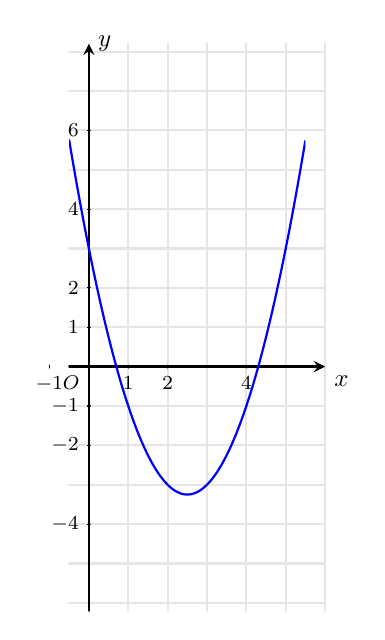
\begin{tikzpicture}[line join=round, line cap=round,>=stealth,thick,scale=0.5]
\tikzset{every node/.style={scale=0.9}}
\draw[gray!20](-0.5,-6.2) grid (6.0,8.2);
\draw[->] (-0.5,0)--(6.0,0) node[below right] {$x$};
\draw[->] (0,-6.2)--(0,8.2) node[right] {$y$};
\draw (0,0) node [below left] {\footnotesize $O$};
 \foreach \x in {-1,1,2,4}
\draw[thin] (\x,1pt)--(\x,-1pt) node [below] {\footnotesize$\x$};
\foreach \y in {-1,1,-4,-2,2,4,6}
\draw[thin] (1pt,\y)--(-1pt,\y) node [left] {\footnotesize$\y$};
\begin{scope}
 \clip (-0.5,-6.2) rectangle (5.5,8.2);
\draw[samples=200,domain=-0.5:5.5,smooth,variable=\x, color=blue] plot (\x,{1*(\x)^2+-5*(\x)+3});
\end{scope}
\end{tikzpicture}

\end{center}

\choice
{ $y=- x^{2} - 5 x - 3$ }
   { $y=x^{2} + 5 x + 3$ }
     { \True $y=x^{2} - 5 x + 3$ }
    { $y=- x^{2} - 5 x + 3$ }
\loigiai{ 

  Đồ thị như hình trên là của hàm số $y=x^{2} - 5 x + 3$. 
 }\end{ex}

\begin{ex}
 Cho tập hợp $A=[-4;1]$ và $B=(-3;2]$ . Tìm ${A\cup B}$. \\ 
\choice
{ \True ${[-4;2]}$ }
   { ${(-3;1]}$ }
     { ${[1;2]}$ }
    { ${[-4;1]}$ }
\loigiai{ 
  
 }\end{ex}

\begin{ex}
 Cho mẫu số liệu như sau: 22; 35; 44; 30; 26; 23; 44; 36; 22; 41; 34; 38. Tính tứ phân vị thứ ba $Q_3$ của mẫu số liệu đã cho.\\ 
\choice
{ \True ${39,5}$ }
   { ${32,92}$ }
     { ${34,5}$ }
    { ${24,5}$ }
\loigiai{ 
  
 }\end{ex}

\begin{ex}
 Cho tam giác ${ABC}$ có $b=2,\widehat{B}=21^\circ, \widehat{C}=27^\circ$. Độ dài cạnh ${a}$ bằng  
\choice
{ ${4,0}$ }
   { \True ${4,2}$ }
     { ${1,6}$ }
    { ${2,5}$ }
\loigiai{ 
 $\widehat{A}=180^\circ-21^\circ-27^\circ=132^\circ$.

$\dfrac{a}{\sin A}=\dfrac{b}{\sin B}\Rightarrow a=\dfrac{b\sin A}{\sin B}=4,2$. 
 }\end{ex}

Trong hệ trục ${Oxy}$, cho hai véctơ $\overrightarrow{c}$ và $\overrightarrow{d}$ có $|\overrightarrow{c}|=10$, $|\overrightarrow{d}|=19$ và góc $(\overrightarrow{c},\overrightarrow{d})=60^\circ$. Tính tích vô hướng $\overrightarrow{c}.\overrightarrow{d}$. 

A. ${\overrightarrow{c}.\overrightarrow{d}=19.5}$.	   B. ${\overrightarrow{c}.\overrightarrow{d}=190}$.	    C. *${\overrightarrow{c}.\overrightarrow{d}=95.0}$.	     D. ${\overrightarrow{c}.\overrightarrow{d}=95 \sqrt{3}}$.


Cho hàm số $f(x)=\left\{ \begin{array}{l} 
     3 x^{2} + 4 x + 6 \text{ khi } x \ge 2  \\ 
     3 - x \text{          khi  } x < 2  
     \end{array} \right.$. Tính $f(-1)$.


A. *${ 4 }$.	   B. $ {2}$.	    C. $ {13}$.	    D. $ {5 }$.


\begin{ex}
 Cho hàm số $y=f(x)$ xác định trên đoạn ${[-2;3]}$ có đồ thị như hình vẽ bên.Tìm tập giá trị của hàm số đã cho.
 
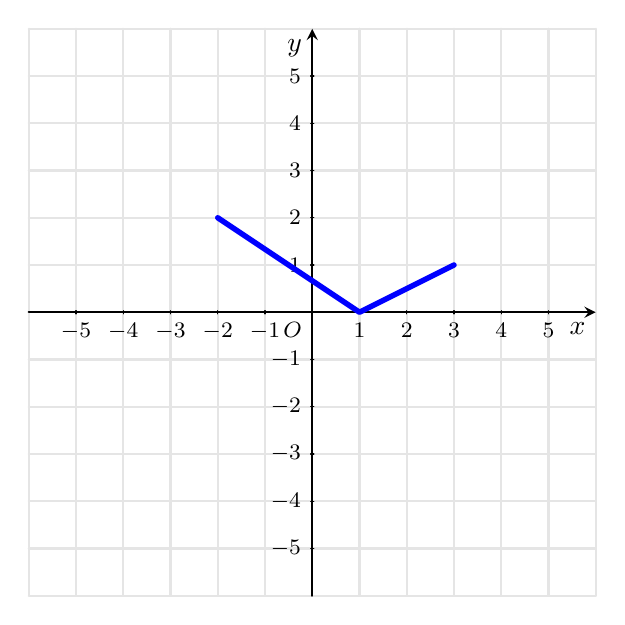
\begin{tikzpicture}[line join=round, line cap=round,>=stealth,thick,scale=0.6]
\tikzset{everynode/.style={scale=0.9}}
\draw[gray!20](-6,-6)grid(6,6);
\draw[->](-6,0)--(6,0)node[below left]{$x$};
\draw[->](0,-6)--(0,6)node[below left]{$y$};
\draw(0,0)node[below left]{\footnotesize$O$};
\foreach \x in{-5,-4,-3,-2,-1,1,2,3,4,5}
\draw[thin](\x,1pt)--(\x,-1pt)node[below]{\footnotesize$\x$};
\foreach \y in{-5,-4,-3,-2,-1,1,2,3,4,5}
\draw[thin] (1pt,\y)--(-1pt,\y)node[left]{\footnotesize$\y$};
\draw[thick,color=blue,line width=2](-2,2)--(1,0)--(3,1);
\end{tikzpicture}
\choice
{ ${[0;5]}$ }
   { ${[-1;4]}$ }
     { ${[-2;2]}$ }
    { \True ${[0;2]}$ }
\loigiai{ 

 Dựa vào đồ thị ta thấy tập giá trị của hàm số là đoạn $[0;2]$. 
 }\end{ex}

\Closesolutionfile{ans}
{\bf PHẦN II. Câu trắc nghiệm đúng sai.}
\setcounter{ex}{0}
\Opensolutionfile{ans}[ans/ans132-2]
\begin{ex}
 Cho mẫu số liệu ${15; 12; 13; 15; 11; 13; 13; 15; 10; 11; 15; 11}$. Xét tính đúng-sai của các khẳng định sau (các kết quả làm tròn đến hàng phần mười):
\choiceTFt
{ Số trung bình của mẫu số liệu là ${13,2}$ }
   { Số trung vị của mẫu số liệu là ${13,5}$ }
     { Mốt của mẫu số liệu là ${12}$ }
    { \True  Khoảng tứ phân vị của mẫu số liệu là 4,0 }
\loigiai{ 
 

 a) Khẳng định đã cho là khẳng định sai.

 $\overline{x}=\dfrac{15+12+13+15+11+13+13+15+10+11+15+11}{12}=12,8$.

b) Khẳng định đã cho là khẳng định sai.

 Sắp xếp dãy số liệu ta được: ${10, 11, 11, 11, 12, 13, 13, 13, 15, 15, 15, 15}$.

Số phần tử là $n=12$ (chẵn) nên trung vị là : $\dfrac{13 +13 }{2}=13=13,0$.

c) Khẳng định đã cho là khẳng định sai.

  Các mốt của mẫu số liệu là: 15.


d) Khẳng định đã cho là khẳng định đúng.

 Tứ phân vị thứ nhất là $Q_1=11,0$.

Tứ phân vị thứ ba là $Q_3=15,0$.

Khoảng tứ phân vị của mẫu số liệu là: $\Delta_Q=15,0-11,0=4,0$.

 
 }\end{ex}

\begin{ex}
 Cho hàm số $f(x)=8 x^{2} + 4 x + 7$. Xét tính đúng sai của các khẳng định sau.
\choiceTF
{ Đồ thị hàm số không đi qua điểm $A(-2;31)$ }
   { Tập xác định của hàm số là khoảng $(-7;+\infty)$ }
     { \True Hàm số đồng biến trên khoảng $\displaystyle \left(- \frac{1}{4};+\infty \right)$ }
    { \True Đồ thị hàm số có hoành độ đỉnh là $\displaystyle x_0=- \frac{1}{4}$ }
\loigiai{ 
 a) Đồ thị hàm số không đi qua điểm $A(-2;31)$ là khẳng định sai vì có $f(-2)=31$ nên đồ thị hàm số đi qua điểm $A(-2;31)$.\\ 
b) Tập xác định của hàm số là khoảng $(-7;+\infty)$ là khẳng định sai vì tập xác định của hàm số là $\mathbb{R}$.\\ 
c) Hàm số đồng biến trên khoảng $\displaystyle \left(- \frac{1}{4};+\infty \right)$ là khẳng định đúng.\\ 
d) Đồ thị hàm số có hoành độ đỉnh là $\displaystyle x_0=- \frac{1}{4}$ là khẳng định đúng.\\ 
 
 }\end{ex}

\Closesolutionfile{ans}
{\bf PHẦN III. Câu trắc nghiệm trả lời ngắn.}
\setcounter{ex}{0}
\Opensolutionfile{ans}[ans/ans132-3]
\begin{ex}
 Tìm số các số nguyên thuộc tập xác định của hàm số $y=\sqrt{128 - 8 x} + \sqrt{10 x + 140}$.
\shortans[oly]{31}

\loigiai{ 
 Điều kiện xác định: 

$\left\{ \begin{array}{l} 
    10 x + 140\ge 0 \\ 
    128 - 8 x\ge 0
    \end{array} \right.$$\Leftrightarrow \left\{ \begin{array}{l} 
    x \ge -14 \\ 
     x \le 16
    \end{array} \right.$$\Rightarrow -14\le x \le 16$.

Tập xác định: $D=\left[-14;16\right]$.

Số các số nguyên thuộc tập xác định là ${31}$. 
 }\end{ex}

\begin{ex}
 Biết đồ thị hàm số $y=ax^2+x+c$ đi qua điểm $C(2;7)$ và nhận đường thẳng $x=- \frac{1}{6}$ làm trục đối xứng. Tính $P=2 a - 2 c$.


\shortans[4]{20}

\loigiai{ 
 Đồ thị hàm số đi qua $C(2;7)$ và $K(-4;37)$ nên ta có:

$\left\{ \begin{array}{l} 
        4 a + c + 2=7 \\ 
        - \frac{1}{2 a}=- \frac{1}{6}
        \end{array} \right.$$\Rightarrow \left\{ \begin{array}{l} 
        4 a + c=5 \\ 
        a=3
        \end{array} \right.$$\Rightarrow \left\{ \begin{array}{l} 
        a=3 \\ 
        c=-7
        \end{array} \right.$

$P=2 a - 2 c=20$. 
 }\end{ex}

\begin{ex}
 Tìm tập xác định của hàm số  $y=\sqrt{x + 5} + \frac{2}{x + 7}$.
 
\loigiai{ 

  Hàm số xác định khi $x + 5\ge 0$ và $x\ne -7$. Suy ra $x \ge -5$. 

 }\end{ex}

\begin{ex}
 Một cửa hàng kinh doạnh mặt hàng A với chi phí sản xuất là ${11}$ triệu đồng và dự định bán ra với giá là ${21}$ triệu đồng. Với giá bán đó, số sản phẩm mà bên khách hàng đối tác sẽ mua trong một năm là ${1110}$ sản phẩm.  Nhằm mục đích đẩy mạnh sản xuất và tiêu thụ sản phẩm này, chủ cửa hàng dự định giảm giá bán và ước tính rằng nếu cứ giảm ${1}$ triệu đồng mỗi sản phẩm thì số lượng sản phẩm bán ra trong một năm sẽ tăng thêm ${185}$ sản phẩm. Cửa hàng phải định giá bán mới của sản phẩm là bao nhiêu, để sau khi thực hiện giảm giá, lợi nhuận thu được sẽ là cao nhất.\ 
\shortans[oly]{${19}$}

\loigiai{ 
  Gọi ${x}$ (triệu đồng) là số tiền dự định giảm giá của sản phẩm ($0 \le x \le 10$) 

 Lợi nhuận thu được khi bán mỗi sản phẩm là $21-x-11=10-x$

 Số sản phẩm mà cửa hàng bán ra trong một năm là $1110+185x$ 

Lợi nhuận mà cửa hàng thu được trong một năm là 

 $f(x)=\left(10 - x\right) \left(185 x + 1110\right)= - 185 x^{2} + 740 x + 11100$ 

${f(x)}$ lớn nhất khi $x=2$ 

 Vậy giá bán mới của mỗi sản phẩm A là ${19}$ triệu đồng thì lợi nhuận thu được cao nhất. 
 }\end{ex}

\Closesolutionfile{ans}

 \begin{center}
-----HẾT-----
\end{center}

 %\newpage 
%\begin{center}
%{\bf BẢNG ĐÁP ÁN MÃ ĐỀ 132 }
%\end{center}
%{\bf Phần 1 }
% \inputansbox{6}{ans132-1}
%{\bf Phần 2 }
% \inputansbox{2}{ans132-2}
%{\bf Phần 3 }
% \inputansbox{6}{ans132-3}
\newpage 




\end{document}